\newpage
\section*{Problem 3:}
Given the matrix description, it is possible to find a reordering (symmetric permutation matrix $P$) that pushes all the non-zero rows to the bottom and all the non-zero columns to the right (except the diagonal entries). The resultant matrix is an \emph{arrow} matrix with $m$ non-zero (dense) rows and columns resides at the bottom-right corner. This is a generalization of the arrow matrix of $m =1$. 

As an example, we take $A \in \mathcal{R}^{n \times n}$, $m= 3$, $n=10$, and $\mathcal{I}=\{2, 6, 8\}$. 


$$
A = 
\begin{bmatrix}
x & x & 0 & 0 & 0 & x & 0 & x & 0 & 0\\
x & x & x & x & x & x & x & x & x & x\\
0 & x & x & 0 & 0 & x & 0 & x & 0 & 0\\
0 & x & 0 & x & 0 & x & 0 & x & 0 & 0\\
0 & x & 0 & 0 & x & x & 0 & x & 0 & 0\\
x & x & x & x & x & x & x & x & x & x\\
0 & x & 0 & 0 & 0 & x & x & x & 0 & 0\\
x & x & x & x & x & x & x & x & x & x\\
0 & x & 0 & 0 & 0 & x & 0 & x & x & 0\\
0 & x & 0 & 0 & 0 & x & 0 & x & 0 & x\\        
\end{bmatrix}
$$

We can permute $A$ with the following permutation matrix 
$$
P = 
\begin{bmatrix}
1 & 0 & 0 & 0 & 0 & 0 & 0 & 0 & 0 & 0\\
0 & 0 & 0 & 0 & 0 & 0 & 0 & 0 & 0 & 1\\
0 & 0 & 1 & 0 & 0 & 0 & 0 & 0 & 0 & 0\\
0 & 0 & 0 & 1 & 0 & 0 & 0 & 0 & 0 & 0\\
0 & 0 & 0 & 0 & 1 & 0 & 0 & 0 & 0 & 0\\
0 & 0 & 0 & 0 & 0 & 0 & 0 & 0 & 1 & 0\\
0 & 0 & 0 & 0 & 0 & 0 & 1 & 0 & 0 & 0\\
0 & 0 & 0 & 0 & 0 & 0 & 0 & 1 & 0 & 0\\
0 & 0 & 0 & 0 & 0 & 1 & 0 & 0 & 0 & 0\\
0 & 1 & 0 & 0 & 0 & 0 & 0 & 0 & 0 & 0\\       
\end{bmatrix}
$$

And the result will be 

$$
P^{T}AP = 
\begin{bmatrix}
x &  0 &  0 &  0 &  0 &  0 &  0 &  x &  x &  x\\
0 &  x &  0 &  0 &  0 &  0 &  0 &  x &  x &  x\\
0 &  0 &  x &  0 &  0 &  0 &  0 &  x &  x &  x\\
0 &  0 &  0 &  x &  0 &  0 &  0 &  x &  x &  x\\
0 &  0 &  0 &  0 &  x &  0 &  0 &  x &  x &  x\\
0 &  0 &  0 &  0 &  0 &  x &  0 &  x &  x &  x\\
0 &  0 &  0 &  0 &  0 &  0 &  x &  x &  x &  x\\
x &  x &  x &  x &  x &  x &  x &  x &  x &  x\\
x &  x &  x &  x &  x &  x &  x &  x &  x &  x\\
x &  x &  x &  x &  x &  x &  x &  x &  x &  x\\       
\end{bmatrix}
$$

The Cholesky factor $L$ of $P^{T}AP$ will thus has the same sparsity structure as $P^{T}AP$ as shown in Figure \ref{fig:mat} for arbitrary $n$ and $m$. Thus, the upper bound of the $nnz(L) = (n-m) + m(n-m) + \frac{1}{2}m^{2}$; where $n - m$ accounts for the diagonal elements (orange line), $m(n-m)$ is the blue rectangle, and $\frac{1}{2}m^{2}$ is the red triangle. 


\begin{figure}[!tbh]
\centering        
   \subfloat {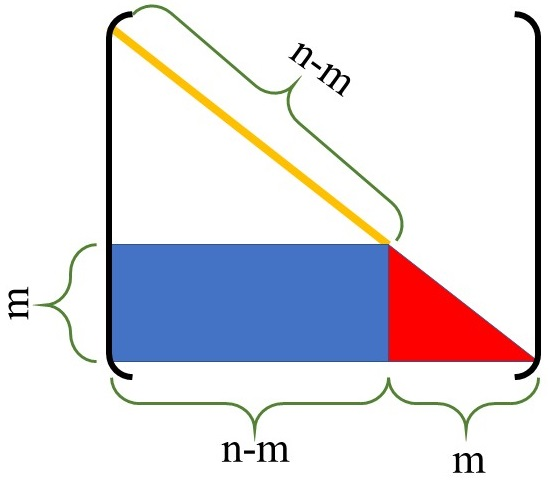
\includegraphics[width=0.65\textwidth]{problem_3.jpg}}
   \caption{Sparsity structure of Cholesky factor $L$}
  \label{fig:mat}
\end{figure}

It is however possible to eliminate the non-zero in the red rectangle due to cancellation. This will give the lower bound of $nnz(L)$ to be $(n-m) + m(n-m)$. 
